We propose a simple, but flexible data processing and analysis framework based entirely on open-source projects, which can run on a local machine. The components of the architecture are illustrated in Figure \ref{fig:architecture}. 

\begin{figure}[h]
    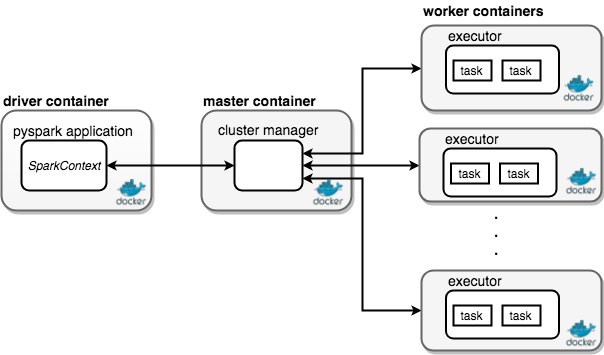
\includegraphics[width=0.45\textwidth]{images/architecture.png}
    \caption{Proposed architecture with standalone Spark cluster in client mode}
    \label{fig:architecture}
\end{figure}

To create and manage independent processing infrastructure we propose to use Docker containers. This enables the application to run on different machines with different operating systems having Docker and Compose installed as the only requirement. 

The containers are started by Docker Compose. The driver container runs the driver applications on the standalone Spark cluster with one or more workers and one master with client deploy mode. In standalone cluster mode, Spark's own cluster manager is used instead of YARN or Mesos. Client deploy mode means that  the driver is launched in the same process as the client that submits the application. 

A master container that deploys Spark master, and one or more worker containers that starts the workers with specified cores and memory, connected to the master. The Spark web user interface shows the available worker on \url{http://localhost:8080}.

For data storage Parquet is recommended over .csv, since most of the operations in the project involve iterating through all rows for given columns. This way we take advantage of the Parquet being an efficient columnar storage. 

Python has become the default programming language for data scientists thanks to packages such as pandas, numpy, and scikit-learn. In big data processing, Apache Spark has become the standard in the recent years. Therefore PySpark is recommended as big data processing and analysis tool.

PySpark DataFrames API is more suitable for processing large amount of data than standard Python packages like Pandas, which cannot handle large data size. PySpark DataFrames have a rich library of functions including string manipulation, date arithmetic, common math operations and they provide a similar interface to DataFrames in Python's Pandas library or to relational tables. \cite{spark-sql}

Standard PySpark data frame operators are translated to SQL queries in the JVM and Spark SQL has information about the structure of both the data and the computation to perform extra optimizations internally. What is more, PySpark DataFrames can be quickly and seamlessly constructed from a different sources such as: structured data files, tables in Hive, external databases, or existing RDDs. \cite{spark-sql} 

In case standard PySpark operators are not sufficient to implement algorithms, Pandas UDFs should be considered instead of row-by-row approach of Spark UDF. In case of the latter, the program needs to iterate over all rows, which results in poor performance in terms of runtime.

This solution can also be scaled for clusters of computers and for cloud computing platforms, such as Amazon Web Services (AWS). Hadoop Distributed File System (HDFS) or Simple Storage Service (S3) in AWS can be integrated for persistent storage. If needed Hadoop's resource manager, YARN can also be added with few changes in the containers.
